% 04-supervised-learning-classification-appendix.tex

% Section Title
\section{SUPERVISED LEARNING - CLASSIFICATION}

    % Main Content

    \subsection{Logistic Regression}

        In this section, we detail the steps and results obtained from using the Logistic Regression model during the supervised learning phase of the project. Logistic Regression served as a baseline model to provide an initial understanding of the classification problem. Despite its simplicity, it offered valuable insights into the multi-label classification task.

        \subsubsection{Model Training \\}

            The Logistic Regression model was trained using its default configuration. Specifically, the \texttt{lbfgs} solver was utilized with a regularization parameter \( C = 1 \). The training process aimed to identify potential overfitting or underfitting issues and establish baseline performance metrics.

                \begin{lstlisting}[caption={Train Logistic Regression model}, label={lst:logistic_regression_train}]
                        # Initialize and train Logistic Regression model
                        model = LogisticRegression(max_iter=1000, random_state=42)
                        model.fit(X_train_tfidf, y_train_binary)
                \end{lstlisting}

            The dataset was preprocessed using the TF-IDF representation of the session texts, which assigned weights to words based on their frequency and relevance within the dataset. Multi-label binary encoding was applied to the `Set\_Fingerprint` column to ensure compatibility with the model.

        \subsubsection{Evaluation Metrics \\}

            The Logistic Regression model was evaluated using standard classification metrics, including weighted F1-scores, precision, and recall. The evaluation metrics highlighted the strengths and weaknesses of the model in handling imbalanced classes. 

                \begin{lstlisting}[caption={Generate classification report}, label={lst:logistic_regression_eval}]
                        # Generate classification report
                        from sklearn.metrics import classification_report
                        report = classification_report(y_test_binary, y_pred, zero_division=0)
                        print(report)
                \end{lstlisting}

            The confusion matrix provided a breakdown of true positives, false positives, false negatives, and true negatives for each intent. Figure~\ref{fig:logistic_cm} shows the confusion matrix for the Logistic Regression model.

            \begin{figure}[H]
                \centering
                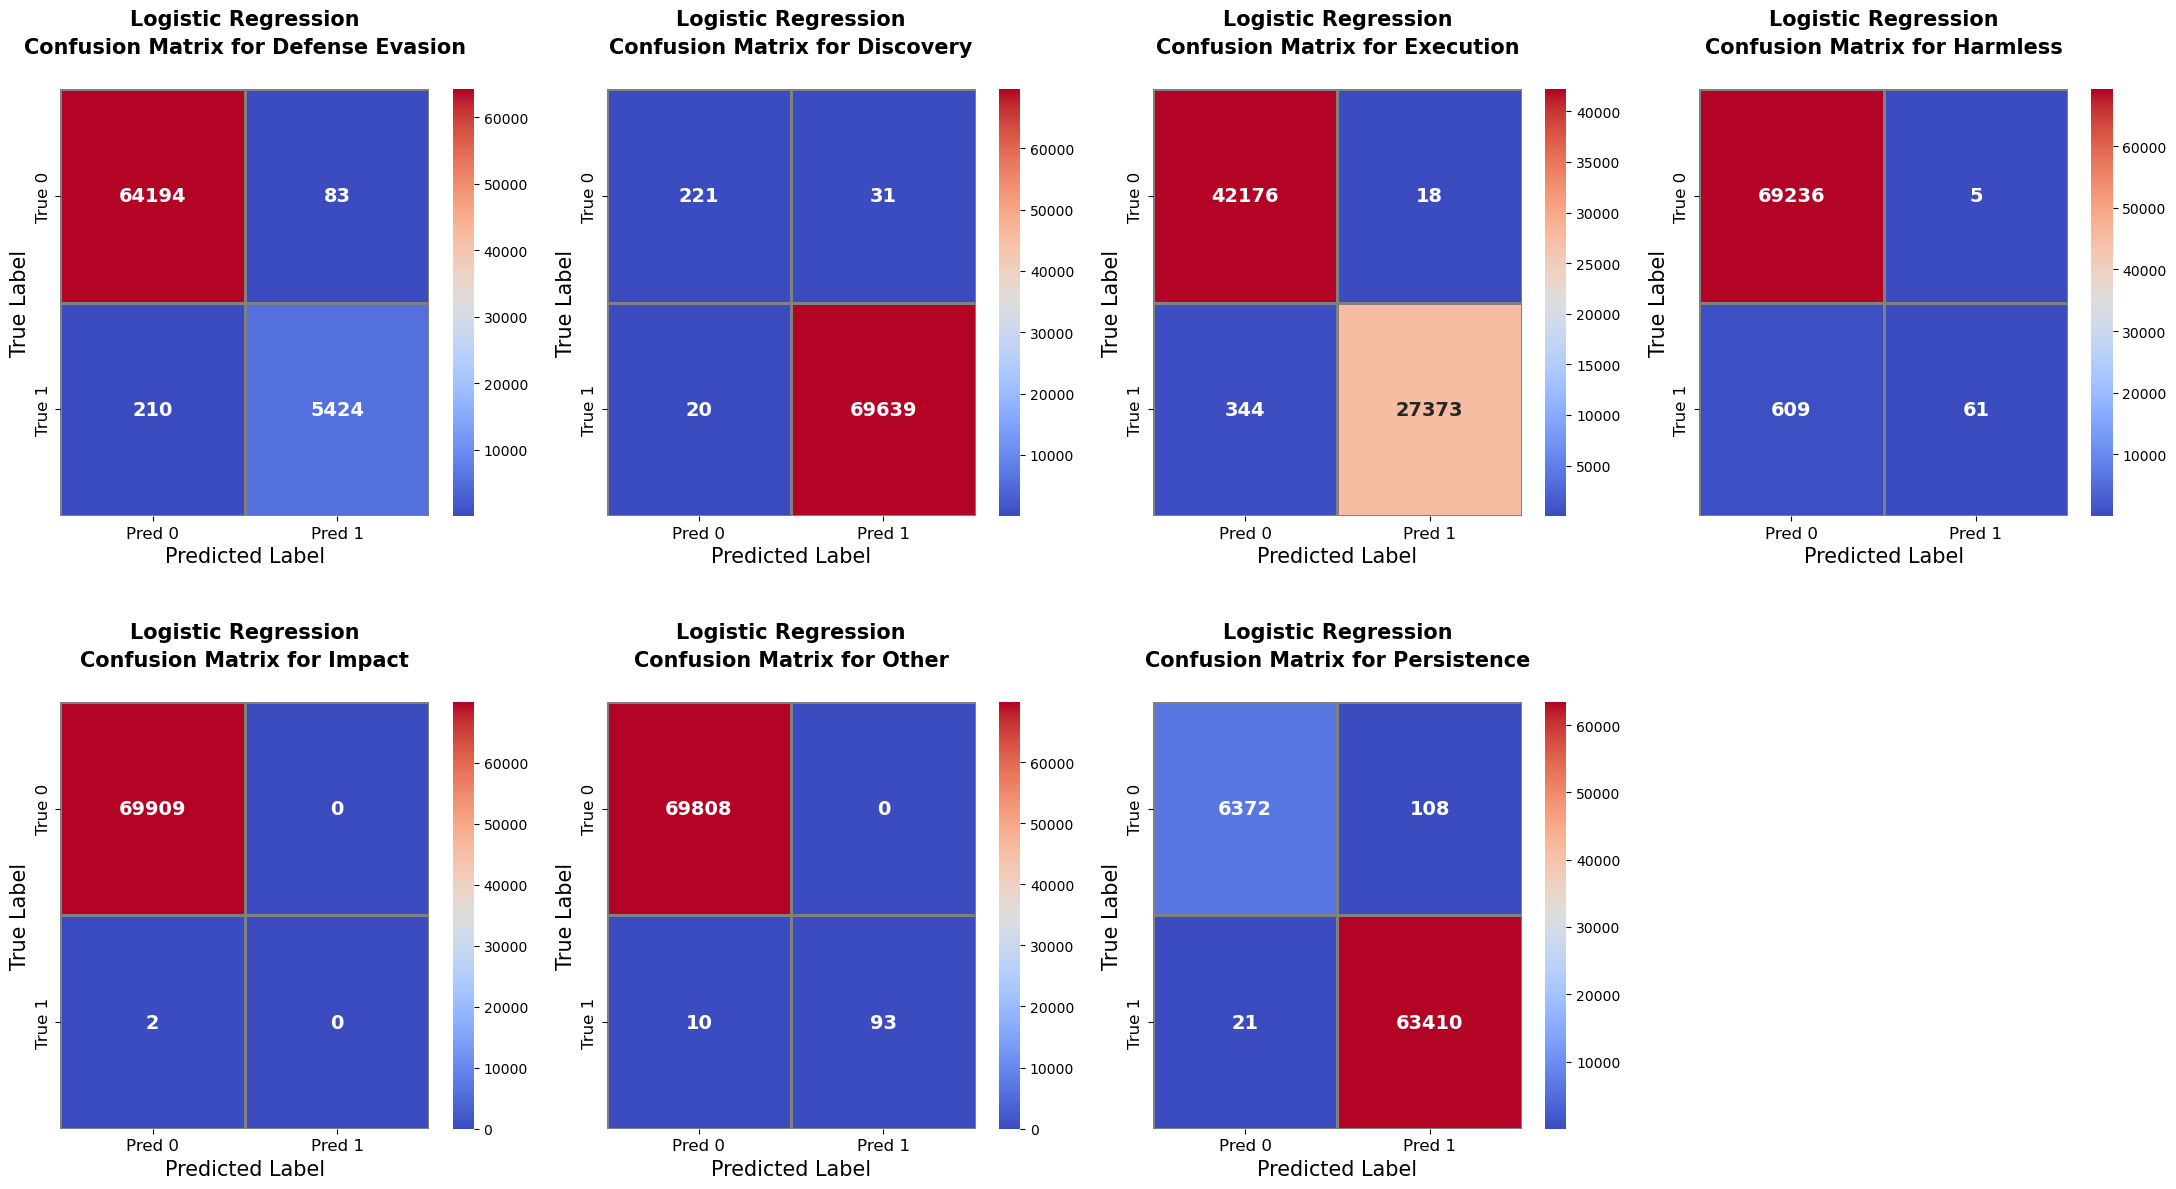
\includegraphics[width=0.8\textwidth]{../figures/plots/section2/Logistic_Regression_confusion_matrices.png}
                \caption{Confusion Matrix for Logistic Regression Model.}
                \label{fig:logistic_cm}
            \end{figure}

        \subsubsection{Hyperparameter Tuning \\}

            Grid search was performed to optimize the Logistic Regression model's hyperparameters. The search focused on varying the regularization parameter \( C \) over a range of values \([0.1, 1, 10, 100]\) to identify the configuration that maximized weighted F1-scores.

                    \begin{lstlisting}[caption={Parameter grid for Logistic Regression}, label={lst:logistic_param_grid}]
                        # Define parameter grid for Logistic Regression
                        param_grid = {'C': [0.1, 1, 10, 100]}
                        grid_search = GridSearchCV(LogisticRegression(max_iter=1000, random_state=42), param_grid, cv=5)
                        grid_search.fit(X_train_tfidf, y_train_binary)
                    \end{lstlisting}

            The optimized model exhibited improved performance compared to the baseline, particularly for intents with smaller sample sizes. Figure~\ref{fig:logistic_tuning} illustrates the weighted F1-scores for different values of \( C \).

            \begin{figure}[H]
                \centering
                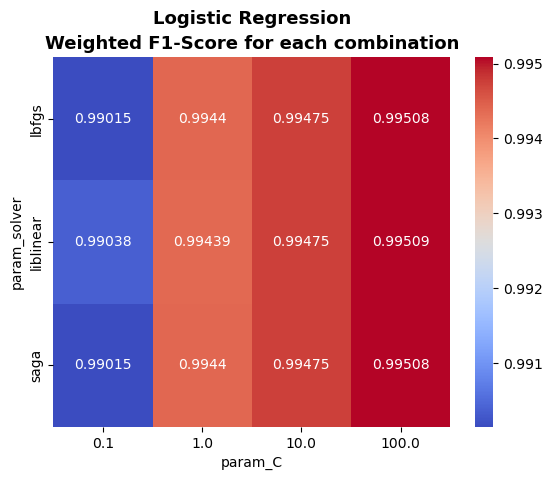
\includegraphics[width=0.8\textwidth]{../figures/plots/section2/weighted_f1_score_for_each_combination_of_parameters_logistic_regression.png}
                \caption{Weighted F1-Scores for Logistic Regression Hyperparameter Tuning.}
                \label{fig:logistic_tuning}
            \end{figure}

        \subsubsection{Comparative Analysis of Baseline and Optimized Models \\}

            The optimized Logistic Regression model demonstrated a moderate improvement in precision and recall compared to the baseline. However, its overall performance remained slightly inferior to more complex models like Random Forest and SVM. The comparative analysis underscores the importance of selecting models suited to the dataset's characteristics and problem requirements.
